\section{Interface 2}

On ne considère désormais le problème qu'a l'interface 2 :

\begin{figure}[!h]
    \centering{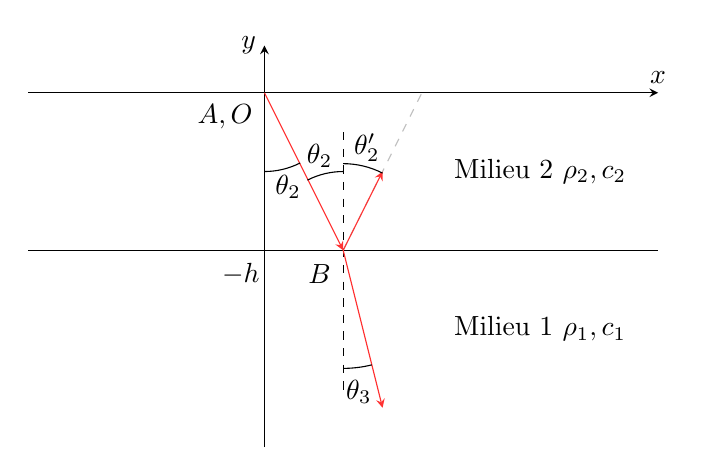
\begin{tikzpicture}

    % ifaces
    \draw [>=stealth, ->] (-3,0) -- (5,0);
    \draw (-3,-2) -- (5,-2);

    % Labels
    \draw (3.5,-1) node {Milieu 2 $\rho_2,c_2$};
    \draw (3.5,-3) node {Milieu 1 $\rho_1,c_1$};

    % verticals
    \draw [dashed] (0,.5) -- (0,-1.5);
    \draw [dashed] (1,-0.5) -- (1,-3.8);

    % axis
    %% y
    \draw [>=stealth, ->] (0,-4.5) -- (0,.6);
    \draw (-.2,.6) node {$y$};
    %% x (already drawn)
    \draw (5,.2) node {$x$};
    %% ordonnée h
    \draw (-.3,-2.3) node {$-h$};


    % points A & B
    \draw (-.5, -.3) node {$A,O$};
    \draw (.7, -2.3) node {$B$};

    % rays
    \draw [red!80, >=stealth, ->] (0,0) -- (1, -2);
    \draw [gray!50, dashed] (1,-2) -- (2,0);
    \draw [red!80, >=stealth, ->] (1,-2) -- (1.5, -1);
    \draw [red!80, >=stealth, ->] (1,-2) -- (1.5, -4);

    % angles
    \draw (0,-1) arc (-90:-63:1) node at (0.3,-1.2) {$\theta_2$};
    \draw (1,-1) arc (90:117:1) node at (.7,-.8) {$\theta_2$};
    \draw (1,-0.9) arc (90:63:1.1) node at (1.3,-.7) {$\theta_2'$};
    \draw (1,-3.5) arc (-90:-76:1.5) node at (1.2,-3.8) {$\theta_3$};


\end{tikzpicture}
}
    \caption{\label{iface2} Considération des effets à l'interface 2}
\end{figure}

\subsection{Position du problème}

\paragraph{Pressions totales}
Dans le milieu 2, la pression totale vérifie :

\begin{equation}
    \left(\Delta - \frac{1}{c_2^2}\frac{\partial^2}{\partial t^2}\right)\pTOT_2(x,y,t) = 0 \;;\; \forall x,t
    \,\mathrm{et}\, \forall y \in [-h; 0] \label{i2_prop1}
\end{equation}

Dans le milieu 1, la pression totale vérifie

\begin{equation}
    \left(\Delta - \frac{1}{c_1^2}\frac{\partial^2}{\partial t^2}\right)\pTOT_1(x,y,t) = 0 \;;\; \forall x,t
    \,\mathrm{et}\, \forall y \leq -h \label{i2_prop2}
\end{equation}

\paragraph{Champ monochromatique} Les ondes sont considérées monochromatiques, l'équation d'Helmholtz est donc vérifiée
dans chacun des milieux :

\begin{eqnarray}
    (\Delta + k_2^2)p_2(x,y) & = & 0 \;;\; \forall x,t \label{i2_helm1}\\
    (\Delta + k_1^2)p_1(x,y) & = & 0 \;;\; \forall x,t \label{i2_helm2}
\end{eqnarray}

\paragraph{Condition de Sommerfeld}

\paragraph{Conditions à l'interface}

A l'interface, il y a continuité des pressions et des vitesses normales. Ainsi :

\begin{eqnarray}
    \pTOT_2(x, y=-h, t) &=& \pTOT_1(x,y=-h,t) \;;\;\forall x,t \label{i2_cl1}\\
    \vTOT_2(x, y=-h, t) &=& \vTOT_1(x,y=-h,t) \;;\;\forall x,t \label{i2_cl2}
\end{eqnarray}

Dans le milieu 1, on ne considérera que l'onde transmise, ainsi pour les equations~\eqref{i2_prop2},~\eqref{i2_cl1}
et~\eqref{i2_cl2}, on aura :

\begin{eqnarray*}
    \pTOT_1 = \pT_1\\
    \vTOT_1 = \vT_1
\end{eqnarray*}

On définit alors :

$$\pTOT_2 = \pI_2 + \pR_2$$

Par ailleurs, on remarque que l'onde incidente à l'interface 2 n'est autre que l'onde transmise depuis l'interface 1, on
a alors :

$$\pI_2 = \pT_1 \Rightarrow \pTOT_2 = \pT_1 + \pR_2$$

De plus, $\pT_1$ est définie par la relation~\eqref{i1_pgent}.

\subsection{Forme générale des pressions}

Les ondes sont considérées monochromatiques :

\begin{eqnarray}
    \pT_1(x,y,t) = \pI_2(x,y,t) & = & A_2e^{j(\omega t-k_2\sin\theta_2x+k_2\cos\theta_2y)} \label{i2_pgeni}\\
    \pR_2(x,y,t) & = & B_2e^{j(\omega t-k_2\sin\theta_2'x+k_2\cos\theta_2'y)} \label{i2_pgenr}\\
    \pT_2(x,y,t) & = & A_3e^{j(\omega_3t-k_1\sin\theta_3x+k_1\cos\theta_3y)} \label{i1_pgent}
\end{eqnarray}

\subsection{Forme générales des vitesses normales}

On sait que les vitesses normales ont une expression de la forme : $v_i(x,y,t) = v_i(x,y)e^{j\omega_it}$, d'après
l'équation d'Euler, on peut écrire les équations~\eqref{i2_euler1} et \eqref{i2_euler2}.

\begin{eqnarray}
    \rho_2\frac{\partial\vTOT_2}{\partial t} = -\frac{\partial\pTOT_2}{\partial y} & \Leftrightarrow & \vTOT_2 =
    -\frac{1}{j\omega\rho_2}\frac{\partial\pTOT_2}{\partial y} \label{i2_euler1}\\
    \rho_1\frac{\partial\vT_1}{\partial t} = -\frac{\partial\pT_1}{\partial y} & \Leftrightarrow & \vT_1 =
    -\frac{1}{j\omega\rho_1}\frac{\partial\pT_1}{\partial y} \label{i2_euler2}\\
\end{eqnarray}

De l'équation~\eqref{i2_euler1} on peut déduire la forme de $\vTOT_2$ (équation~\eqref{i2_vgentot}), et
de~\eqref{i2_euler2} on déduit~\eqref{i2_vgent}.

\begin{eqnarray}
    \vTOT_2 & = & -\frac{1}{j\rho_2\omega}\left[jA_2k_2\cos\theta_2e^{j(\omega t-k_2\sin\theta_2x+k_2\cos\theta_2y)}
        - jB_2k_2\cos\theta_2'e^{j(\omega t - k_2\sin\theta_2'x-k_2\cos\theta_2'y)}\right]\notag\\
    & = & -\frac{1}{\rho_2\omega}\left[A_2k_2\cos\theta_2e^{j(\omega t-k_2\sin\theta_2x+k_2\cos\theta_2y)}
        - B_2k_2\cos\theta_2'e^{j(\omega t - k_2\sin\theta_2'x-k_2\cos\theta_2'y)}\right] \label{i2_vgentot}
\end{eqnarray}

\begin{eqnarray}
    \vT_2
        & = &
    -\frac{1}{j\rho_1\omega_3}\left[jA_3k_1\cos\theta_3e^{j(\omega_3t-k_1\sin\theta_3x+k_1\cos\theta_3y)}\right]\notag\\
        & = &
    -\frac{1}{\rho_1\omega_3}\left[A_3k_1\cos\theta_3e^{j(\omega_3t-k_1\sin\theta_3x+k_1\cos\theta_3y)}\right] \label{i2_vgent}
\end{eqnarray}

\subsection{Conditions aux limites}

\subsubsection{Continuité des pressions}

On a 

\begin{equation*}
\eqref{i2_cl1} \Leftrightarrow \pTOT_2(x,y=-h,t) = \pT_2(x, y=-h, t) \;;\; \forall x,t 
\end{equation*}

Ainsi, en insérant~\eqref{i2_pgeni},~\eqref{i2_pgenr} et~\eqref{i2_pgent} dans~\eqref{i2_cl1}, on obtient
l'équation~\eqref{i2_cl1_insert}.

\begin{eqnarray}
    A_2e^{j\omega t}e^{-jk_2\sin\theta_2x}e^{-jk_2\cos\theta_2h} + B_2e^{j\omega t}e^{-jk_2\sin\theta_2'x}e^{jk_2\cos\theta_2'h} & = &
    A_3e^{j\omega_3t}e^{-jk_1\sin\theta_3x}e^{-jk_1\cos\theta_3h} \label{i2_cl1_insert}
\end{eqnarray}

On veut que~\eqref{i2_cl1_insert} soit valable pour tout $t$, on a alors :

\begin{eqnarray}
    e^{j\omega t} = e^{j\omega_3t} & \Leftrightarrow &\omega = \omega_3 = \omega \label{i2_pulsrel}
\end{eqnarray}

On veut aussi que~\eqref{i2_cl1_insert} soit valable pour tout $x$, on a alors :

\begin{eqnarray}
    e^{-jk_2\sin\theta_2x} = e^{-jk_2\sin\theta_2'x} & = & e^{-jk_1\sin\theta_3x}\notag\\
    \text{d'où}\;\theta_2 & = & \theta_2'\label{i2_thetarel}\\
    e^{-jk_2\sin\theta_2x} & = & e^{-jk_1\sin\theta_3x}\notag\\
    \Leftrightarrow k_2\sin\theta_2 & = & k_1\sin\theta_3 \label{i2_snellrel}
\end{eqnarray}

A FINIR
